\documentclass[spanish]{beamer}

%Language symbols
\usepackage[spanish]{babel}
\selectlanguage{spanish}
\usepackage[utf8]{inputenc}
\usepackage{verbatim}

\usepackage{graphicx}
\usepackage{subfig}


\usepackage{algorithm}
\usepackage{algpseudocode}
\usepackage{pifont}

\usepackage{movie15}
% Code

\usepackage{listings,textcomp}
\lstset{
  breakatwhitespace,
  language=c++,
  columns=fullflexible,
  keepspaces,
  breaklines,
  tabsize=2, 
  showstringspaces=false,
  extendedchars=true,
  basicstyle=\fontfamily{pcr}\selectfont\scriptsize,
  keywordstyle=\color{orange},
  upquote=true,
  literate={-}{-}1}

%Theme
\usetheme{metropolis}

%Title
\title{Problema del viajante de comercio\\
Travelling salesman problem}
\date{\today}
\author{José Antonio Álvarez Ocete \\ Norberto Fernández de la Higuera \\ Javier Gálvez Obispo \\ Yábir García Benchakhtir}
\institute{Doble Grado en Ingeniería Informática y Matemáticas}
%Document
\begin{document}

\frame{\titlepage}

\begin{frame}\frametitle{Descripción del problema}

  \begin{figure}[H]
    \centering
    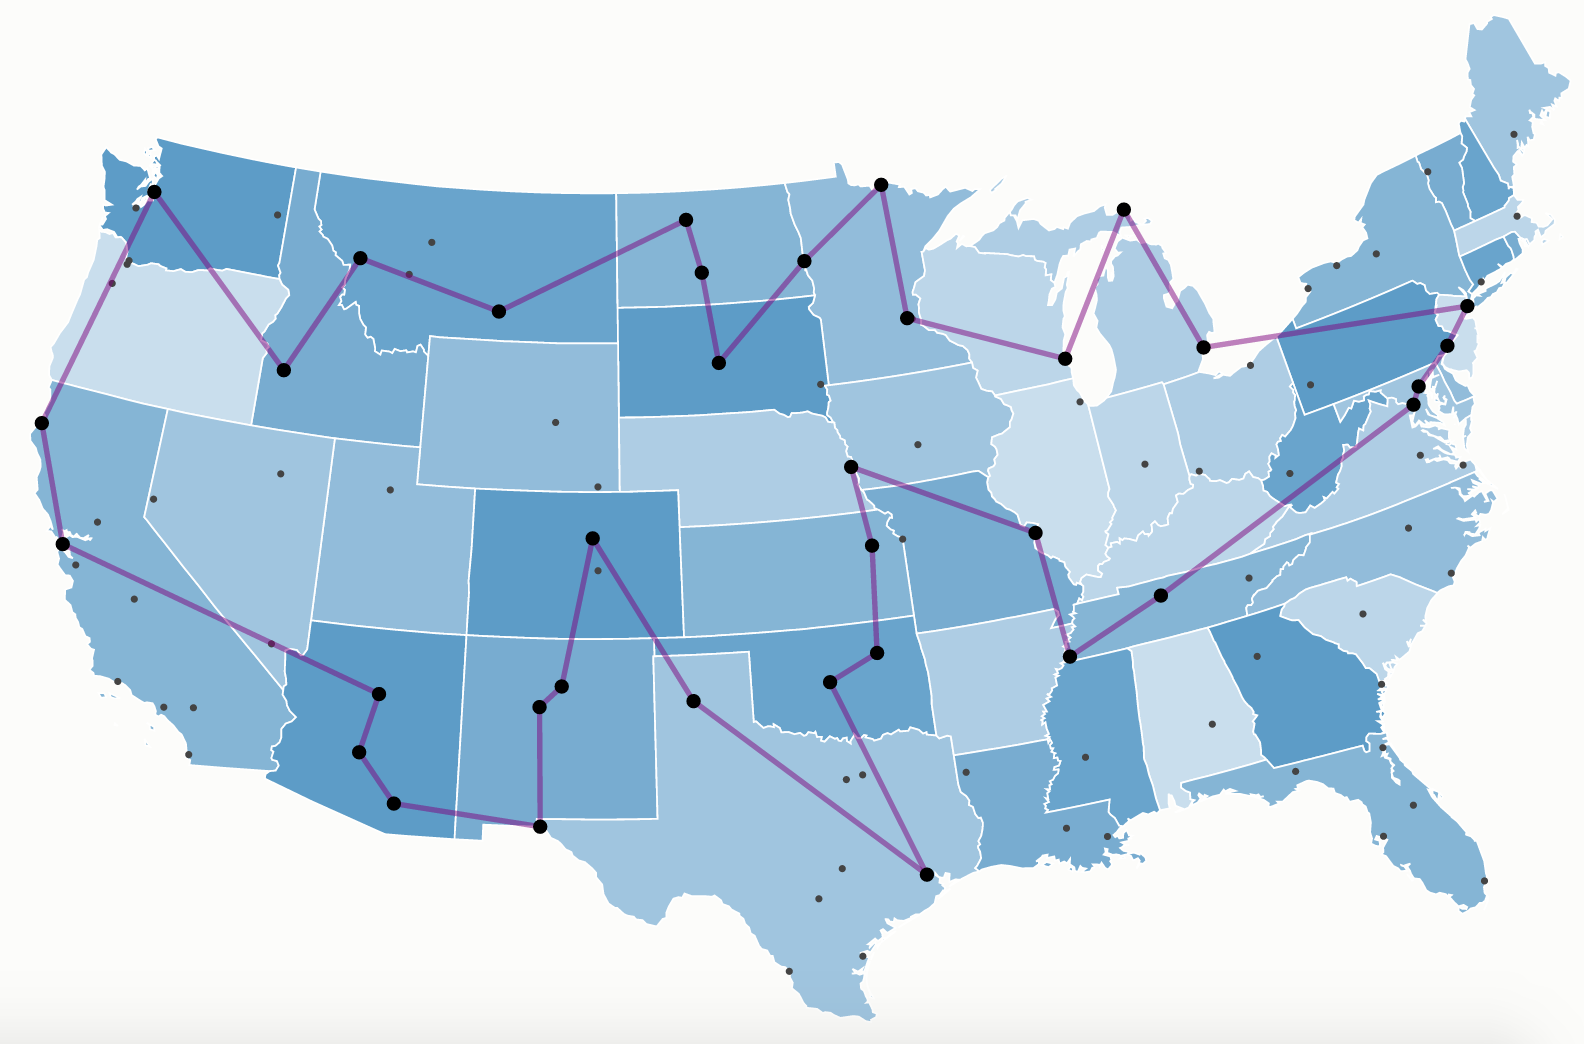
\includegraphics[width=0.8\textwidth]{mapa.png}
  \end{figure}
  
\end{frame}

\begin{frame}\frametitle{Vecino más cercano}
  
  \begin{algorithm}[H]
    \caption{Nearest Neighbor}
    \begin{algorithmic}
      \State $\mathcal{R}$ = [random(0,$|$ $\Omega$ $|$)]
      \State $\mathcal{C}$ - $\mathcal{R}$[0]
      \For{pos in [0,n-2]}
      \State bestPos = nearest($\mathcal{M}$[$\mathcal{R}$[pos]],$\mathcal{C}$)
      \State $\mathcal{R}$.push($\mathcal{C}$[bestPos])
      \State $\mathcal{C}$.erase(bestPos)
      \EndFor
      \State return $\mathcal{R}$
    \end{algorithmic}
  \end{algorithm}

\end{frame}

\begin{frame}\frametitle{Ejemplo de ejecución}
  \includemovie{1cm}{1cm}{nearest.gif}
  \footnote[1]{Si no se muestra correctamente se adjunta el ejemplo en el archivo nearest.gif}
  \footnote[2]{También está disponible en \href{https://imgur.com/a/8DiZvby}{https://imgur.com/a/8DiZvby}}
\end{frame}

\begin{frame}\frametitle{Insercción de minimo coste}
  \begin{algorithm}[H]
    \caption{Cheap Insert}
    \begin{algorithmic}
      \State i, j = nodes(min($M$))
      \State path = [i, j]
      \State $\mathcal{C}$ = $\Omega$ - path
      \While{C not empty}
      \For{city in cities}
      \If{city not in path}
      \For{node in path}
      \State T = minimizeDistance(node, city, node+1)
      \EndFor
      \State insert(path, T)
      \State remove($\mathcal{C}$, T)
      \EndIf
      \EndFor
      \EndWhile
      \State return path
    \end{algorithmic}
  \end{algorithm}
  
\end{frame}

\begin{frame}\frametitle{Ejemplo de ejecución}
  \includemovie{1cm}{1cm}{cheap.gif}
  \footnote[1]{Si no se muestra correctamente se adjunta el ejemplo en el archivo cheap.gif}
  \footnote[2]{También está disponible en \href{https://imgur.com/a/8DiZvby}{https://imgur.com/a/8DiZvby}}
\end{frame}

\begin{frame}\frametitle{Insercción del más lejano}
  \begin{algorithm}[H]
    \caption{Cheap Insert}
    \begin{algorithmic}
      \State i, j = nodes(max($M$))
      \State path = [i, j]
      \State $\mathcal{C}$ = $\Omega$ - path
      \While{C not empty}
      \For{city in cities}
      \If{city not in path}
      \For{node in path}
      \State T = maximize(node, city, node+1)
      \EndFor
      \State insert(path, T)
      \State remove($\mathcal{C}$, T)
      \EndIf
      \EndFor
      \EndWhile
      \State return path
    \end{algorithmic}
  \end{algorithm}
\end{frame}

\begin{frame}\frametitle{Ejemplo de ejecución}
  \includemovie{1cm}{1cm}{furthest.gif.gif}
  \footnote[1]{Si no se muestra correctamente se adjunta el ejemplo en el archivo furthest.gif}
  \footnote[2]{También está disponible en \href{https://imgur.com/a/8DiZvby}{https://imgur.com/a/8DiZvby}}
\end{frame}


\end{document}

